\documentclass{article}

\usepackage[english]{babel}
\usepackage[letterpaper,top=2cm,bottom=2cm,left=3cm,right=3cm,marginparwidth=1.75cm]{geometry}
\usepackage{tikz}
\usetikzlibrary{arrows.meta, positioning}

\title{Advanced Computer Architecture\\Homework 1: Multithreading AlphaBot2}
\author{
    Philipp Dietle\\
    Matriculation ID: \texttt{TODO}
    \and
    Lorenz Scherrer\\
    Matriculation ID: \texttt{TODO}
    \and
    Gioele Pettarini\\
    Matriculation ID: \texttt{TODO}
}
\date{
    Group: \texttt{TODO}
    \quad
    Robot: 8
}

\begin{document}
\maketitle

\section{Introduction}

The goal of this assignment is to coordinate the AlphaBot2's main tasks so that the robot can complete a round trip on the black track while also reacting to objects in its environment. The required tasks are:
\begin{enumerate}
    \item continuously following the black line without veering off the track;
    \item detecting obstacles with the infrared sensors and buzzing once, twice, or three times for the first, second, or third detected object;
    \item recognizing a shoe, a bottle, and a mug with the camera, then setting the RGB LED to red, yellow, or green respectively.
\end{enumerate}

The main challenge is that these tasks have very different timing requirements. Line following must react frequently to keep the robot stable, while camera-based object recognition is much slower and can block the control loop if executed sequentially.

\section{Naive approaches}

Our first version kept the whole behavior in one loop. The robot read the line sensors, checked the infrared sensors, ran camera recognition, and then updated the outputs. On the track this failed quickly. During a recognition step the motors kept their previous command for too long, so the robot started drifting before the next line correction.

We then tried to fix the drift by changing only the line-following controller. We added integral and derivative terms and tuned the constants, but the result was not stable enough. The extra terms sometimes made the corrections too strong. They also did nothing while recognition was blocking the loop. After that test we used a simpler proportional controller again, because the timing problem was larger than the controller-tuning problem.

After that we split the program into Python threads for driving, camera recognition, and infrared obstacle detection. The code matched the three tasks better, but the robot still had pauses. The vision thread competed for CPU time with the driving thread, and Python's Global Interpreter Lock (GIL) limits how much CPU-bound Python code can run at the same time. We also had small coordination bugs in the first threaded versions: the stop flag and object counter were shared informally, and the buzzer loop could keep running while the rest of the robot should already have moved on.

We also tested separate processes to move the expensive recognition work away from the control loop. That avoided the GIL for recognition, but the robot hardware did not fit this version well. The camera, GPIO pins, model, and AlphaBot object could not be treated as shared objects. Each process had its own memory, so state such as the stop condition, the detected-object count, and the latest recognition result had to be passed explicitly. The first multiprocessing version was harder to debug than the threaded one and overall ended up not working.

For the final version, we kept one rule from these failed attempts: the driving loop should do only line sensing and motor updates. Recognition, buzzing, and LED updates can run outside that loop, but they should exchange only the few values the driver actually needs.

\section{Benchmarking}

We already knew that object recognition was the heaviest computation, but we wanted real numbers to use when designing the final solution. For this reason, we benchmarked the main operations.
The measured runtimes are summarized here.

\begin{center}
\begin{tabular}{lrr}
\hline
Task & Iterations & Average time per iteration \\
\hline
Line following & 100 & 0.009808 s \\
Object recognition & 30 & 0.245612 s \\
Infrared obstacle check & 100 & 0.000425 s \\
\hline
\end{tabular}
\end{center}

The measurements confirmed our expectation and gave us a concrete starting point for the redesign. Object recognition takes about 0.25 seconds per iteration, while line following and infrared checking are much shorter. In the sequential version, every recognition step therefore skipped many possible line-following updates, which explains the drifting behavior we observed on the track.

\section{Solution Design}

The final program keeps the fast robot control in the main process and moves the camera work out of it. The main process creates the \texttt{AlphaBot2} object only after the camera and vision processes have reported that they are ready. GPIO writes, PWM motor commands, infrared reads, buzzer control, and LED updates stay in one place instead of being spread across processes.

Camera capture and recognition use two separate processes. The camera process starts CameraServer with a frame queue. We changed CameraServerClass.py so it can receive this optional queue. Its capture thread still updates the latest frame for the web stream, and it also pushes a frame into the queue. The queue has size one, so an old frame is dropped if the vision process is still busy. We prefer a recent frame over a backlog of old frames.

The vision process loads MobileNet once. It limits Torch to one thread, reads frames from the frame queue, and maps ImageNet IDs to \texttt{shoe}, \texttt{bottle}, or \texttt{mug}. It writes the newest result to a result queue, also with size one. The main loop checks that queue without blocking. When a label is available, the LED is set according to the assignment: shoe red, bottle yellow, and mug green.

\begin{center}
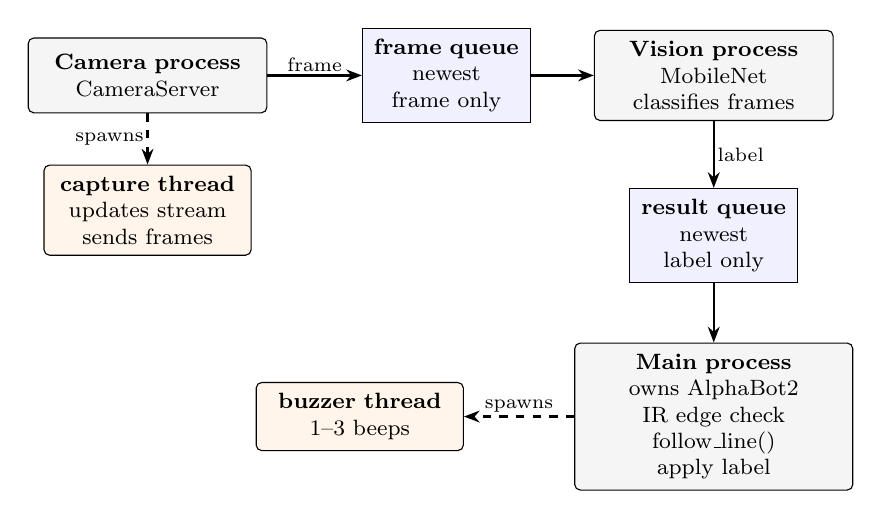
\begin{tikzpicture}[
    font=\footnotesize,
    node distance=0.65cm and 0.8cm,
    process/.style={
        draw,
        rounded corners=2pt,
        align=center,
        fill=gray!8,
        minimum height=0.95cm,
        text width=2.75cm,
        inner sep=4pt
    },
    queue/.style={
        draw,
        align=center,
        fill=blue!6,
        minimum height=0.85cm,
        text width=1.85cm,
        inner sep=4pt
    },
    thread/.style={
        draw,
        rounded corners=2pt,
        align=center,
        fill=orange!8,
        minimum height=0.75cm,
        text width=2.35cm,
        inner sep=4pt
    },
    comm/.style={-{Stealth[length=2mm]}, thick},
    spawn/.style={-{Stealth[length=2mm]}, thick, dashed}
]
    \node[process] (camera) {\textbf{Camera process}\\CameraServer};
    \node[queue, right=1.2cm of camera] (frameq) {\textbf{frame queue}\\newest frame only};
    \node[process, right=of frameq] (vision) {\textbf{Vision process}\\MobileNet\\classifies frames};
    \node[queue, below=0.85cm of vision] (resultq) {\textbf{result queue}\\newest label only};
    \node[process, below=0.75cm of resultq, text width=3.25cm] (main) {
        \textbf{Main process}\\
        owns AlphaBot2\\
        IR edge check\\
        follow\_line()\\
        apply label
    };
    \node[thread, below=0.65cm of camera] (capture) {
        \textbf{capture thread}\\
        updates stream\\
        sends frames
    };
    \node[thread, left=1.4cm of main] (beep) {
        \textbf{buzzer thread}\\
        1--3 beeps
    };

    \draw[comm] (camera) -- node[midway, above, font=\scriptsize, fill=white, inner sep=1pt] {frame} (frameq);
    \draw[comm] (frameq) -- (vision);
    \draw[comm] (vision) -- node[midway, right, font=\scriptsize, fill=white, inner sep=1pt] {label} (resultq);
    \draw[comm] (resultq) -- (main);
    \draw[spawn] (camera) -- node[midway, left, font=\scriptsize, fill=white, inner sep=1pt] {spawns} (capture);
    \draw[spawn] (main.west) -- node[midway, above, font=\scriptsize, fill=white, inner sep=1pt] {spawns} (beep.east);
\end{tikzpicture}
\end{center}

Obstacle detection remains in the main process because it is cheap and tied to the buzzer. We keep \texttt{obstacle\_was\_present} to count only the edge of an obstacle; otherwise the same object would be counted many times while it stayed in front of the sensor. The buzzer pattern runs in a short thread, so beeping does not stop \texttt{follow\_line} from being called.

We use processes only for the two parts that can delay driving: grabbing frames and running the neural network. The loop that steers the robot stays fast: infrared check, possible buzzer trigger, \texttt{follow\_line}, optional LED update, and a 1 ms sleep. The queues carry frames and classification dictionaries; they never carry the \texttt{AlphaBot2} object.

\section{Results (heavy revision needed / missing contents)}

The final implementation should be evaluated against the assignment requirements:
\begin{enumerate}
    \item ability to follow the track with at most one slight deviation;
    \item correct recognition of the shoe, bottle, and mug;
    \item correct buzzer behavior for the first, second, and third detected object;
    \item correct RGB LED colors: red for the shoe, yellow for the bottle, and green for the mug;
    \item round-trip time on the track.
\end{enumerate}

Compared with the sequential implementation, the expected improvement comes from preventing camera recognition from blocking line following. The benchmark results support this design decision because recognition is approximately 25 times slower than one line-following iteration.

\section{Conclusion (heavy revision needed / missing contents)}

The sequential implementation showed that object recognition cannot be placed directly in the main control loop without harming navigation. Benchmarking identified camera inference as the dominant cost, while line following and infrared checks were comparatively lightweight. The final solution therefore separates the time-critical control loop from slower background tasks and uses shared state only for the information needed by the buzzer and LED behavior.

\end{document}
